% Documentclass options:
%    10pt, 11pt, 12pt  -- set type size
%    draft             -- single space, mark overfull hboxes on paper
%    final             -- double space, don't mark overfull hboxes on paper
%    oneside           -- format for one-sided printing
%    twoside           -- format for two-sided printing
% Defaults are 11pt,final,oneside.  Keep these, please.
\documentclass[11pt]{ucscthesisbs}
\bibliographystyle{apalike2}
\usepackage{natbib}
\usepackage{graphicx,epsf}% Include figure files
\usepackage{spverbatim}
\newcommand{\aj}{Astronomical Journal}
\newcommand{\apj}{Astrophysical Journal}
\newcommand{\icarus}{Icarus}
\newcommand{\aap}{Astronomy and Astrophysics}     % Astronomy and Astrophysics 
\newcommand{\mnras}{Monthly Notices of the Royal Astronomical Society} 
\newcommand{\nat}{Nature} 
\newcommand{\jgr}{Journal of Geophysical Research}

% The following declaration is for citations and bibliographies consistent with
% Astrophysical Journal specifications.  It may be left out or replaced with
% another bibliography/citation style.  See also the "\bibliographystyle"
% command later in this file.
%\usepackage{apj}

\usepackage{xcolor}
\usepackage{pagecolor}
\usepackage{lipsum}  
\usepackage{subfig}
\usepackage{amsmath}
\usepackage[font=small,labelfont=bf]{caption}


% \pagecolor{darkgray}
% \color{white}

\pagecolor{white}
\color{black}


\begin{document}

% Declarations for Front Matter

\title{Thermal Evolution of Uranus and Neptune with Condensation-inhibited Convection}
\author{Robert Schroder}
\degreeyear{2020}
\degreemonth{December}
\degree{BACHELOR OF SCIENCE}
\field{ASTROPHYSICS}%

% Declare up to five committee members.  The text will be reproduced directly
% on the signature page.  Though the chair is a committee member, leave
% him/her out of the \committeemember declarations.  Make sure \numberofmembers
% agrees with the number of committee members declared INCLUDING the chair.
% If it is wrong, you will get extra or missing lines on the signature page.
%
\chair{Bruce Schumm}
\thesisadvisor{Christopher Mankovich}
\technicaladvisor{Jonathan Fortney}
\numberofmembers{2}




\campus{Santa Cruz}

\maketitle
\copyrightpage

\begin{frontmatter}

\begin{abstract}
This will be the last section written, once we have finished our results and conclusion.
\end{abstract}

\tableofcontents
%
% The most recent (10/95) guidelines make absolutely no mention of the list
% of figures and list of tables.  Are they necessary?  If not, comment the
% next two lines out.
%
\listoffigures
\listoftables


\end{frontmatter}

%\part{First Part}

\chapter{Introduction}
Planets coalesce from matter contained in their parent star's protoplanetary disk. As planets accrete material from the disk, it heats up, giving the planet a so-called 'hot start'. After accretion is complete, the planet will begin to cool over time. It will be helpful to define what we mean by temperature. There are several temperatures that describe a planet's atmosphere. The effective temperature, $T_{\rm eff}$, is defined as the total flux integrated over all frequencies of a black body of the same shape and same distance as the planet \citep{seager_2010}.
\begin{equation}
    \pi \int_{0}^{\infty} B(T, \nu) d\nu = \sigma_{\rm R}T^{4}
  \label{eq:effective_temp_integral}
\end{equation}  
yielding,
\begin{equation}
    T_{\rm eff} = \bigg(\frac{F}{\sigma_{\rm R}}\bigg)^{\frac{1}{4}} 
  \label{eq:effective_temp}
\end{equation} 
The equilibrium temperature, $T_{\rm eq}$, is the temperature the planet would have if it were in thermal equilibrium with its parent star. This occurs when the planet has radiated away its latent heat of formation, and the only remaining source of energy is from its star. This temperature is defined as:
\begin{equation}
    T_{\rm eq}^4 = \frac{F(1-A_{\rm B})}{r^{2} 4 \pi \sigma_{\rm B}}
  \label{eq:equilibrium_temp}
\end{equation} 
where $r$ is the distance from the star in AU, $A_{\rm B}$ is the bond albedo, and $F$ is the solar flux. Finally, the intrinsic temperature, $T{\rm int}$, the temperature that defines the flux from the planet's interior and is defined by the relation:

\begin{equation}
    T_{\rm eff}^4 =  T_{\rm eq}^4 +  T_{\rm int}^4
  \label{eq:effective_temp}
\end{equation} 

In 1965, Frank Low measured Jupiter's intrinsic temperature \citep{low_1966}. To explain this observation, theorists set out to expand on prior work \citep{demarcus_1958} on the theory of interior structure of solar system gas and ice giants \citep{hubbard_1968, smoluchowski_1967,hubbard_1977, hubbard_1977_2, podolak_1991}. Models have assumed that the interior of giant planets are convective, meaning that heat within the planet's interior is transferred by the movement of fluids. More specifically, warmer, less dense material will rise; while cooler, more dense material will sink due to the influence of gravity. In 1968, Hubbard showed that a convective interior would allow Jupiter's observed flux to be transported to the surface adiabatically. This analysis motivated the inclusion of adiabatic interiors in contemporary interior structure models for gas and ice giants.

At the present time, most of the giant planets in our solar system: Saturn, Jupiter, and Neptune, all have an intrinsic flux. Uranus is the exception \citep{pearl_conrath_1991}. Measurements of Uranus's effective temperature are consistent with a planet that has no intrinsic flux, a planet in thermal equilibrium with the Sun, cooler than its more distant neighbor, Neptune, a planet with similar mass and composition. 

While thermal evolution models do currently reproduce $T_{\rm eff}$ for Jupiter and Neptune at 4.6 Gyr \citep{graboske_1975,fortney_2011}, they do not reproduce $T_{\rm eff}$ for Saturn and Uranus. Models for Saturn predict a cooler planet; however, plausible explanations have been offered to explain its current, warmer $T_{\rm eff}$. Among them, the rain-out of helium \citep{fortney_hubbard_2003, mankovich_2020}, or double-diffusive convection \citep{leconte_chabrier_2013}. 

Meanwhile, for Uranus, the models have predicted a warmer effective temperature at present time \citep{fortney_2011, podolak_1991, hubbard_1995, scheibe_2019}. There have been various attempts to explain Uranus' cool temperature. Early investigations posited that a stratified interior, stable against convection, would allow heat to be trapped deep within the the interior \citep{podolak_1991}. If the interior were stable against convection, some other means of energy transport must be responsible for transporting heat from the interior to the surface. Later work investigated possible mechanisms for energy transport other than dry,adiabatic convection. [NEED TO WORK ON THIS] The formation of stable condensation zones \citep{friedson_2017}, \citep{leconte_2017}, and \citep{guillot_1995}, and thermal boundary layers \citep{nettelmann_2016}, that could inhibit convection. It was speculated that the presence of these thermal boundary layers, or condensation zones, could trap heat deep within the interior, allowing the envelope above to cool more rapidly, thereby lowering the planet's effective temperature.

\section{Condensation in Hydrogen Dominated Atmospheres}
Up to now, we have discussed convection, but we haven't explicitly called it dry convection. When we speak of dry convection, we are not taking into consideration the condensation of molecular species in the atmosphere. On Earth, the atmosphere undergoes moist convection. As a parcel of air is lifted, it cools until it gets cold enough that water vapor condenses out, releasing latent heat of condensation which boosts convection. This release of latent heat alters the temperature-pressure profile, which now follows a moist adiabat.  In addition to the temperature gradient, there may also be a gradient in mean molecular weight. On Earth, moist air is lighter than dry air. For example, H$_{2}$O vapor (molecular mass = 18 g/mol), the primary condensate in Earth's atmosphere is lighter (not by much) than the background air which is composed primarily of N$_{2}$ (molecular mass = 28 g/mol). When H$_{2}$O vapor abundance exceeds the saturation vapor pressure, the vapor condenses out of the atmosphere, resulting in a small vertical gradient in mean molecular weight. In Earth's atmosphere, this small gradient does not impose a significant barrier to convection. By contrast, in hydrogen dominated atmospheres such as Neptune and Uranus, the background gas is much lighter than the condensates. In this hydrogen-rich environment, when H$_{2}$O condenses out of the atmosphere, a strong vertical gradient in mean molecular weight can be established, resulting in a negative buoyancy for the convecting parcel of gas. This can create a situation where the zone in which water condenses is stable against convection \citep{guillot_1995}, \citep{friedson_2017}, \citep{leconte_2017}. Thus far, we have been discussing H$_{2}$O as the only condensate. However, other condensates such as NH$_{3}$ and CH$_{4}$ may impact convection as well. In this study, we consider H$_{2}$O as the primary condensate as it likely has the largest impact. The reason for this is that if its abundance is supercritical, then it results in a larger superadiabicity (larger temperature gradient) than would be provided by either NH$_{3}$ r CH$_{4}$ \citep{guillot_1995}. Consideration of other condensates is planned for future work.

The work done by \citep{guillot_1995}, \citep{friedson_2017}, and \citep{leconte_2017} examined under what conditions stable condensation zones would form. In this paper, we apply the same physical mechanisms for the formation of stable water condensation zones. However, we expand on this by placing the formation of these stable, radiative layers in the context of a more complete model of interior structure for solar system ice giants. Furthermore, we investigate how these stable layers impact the cooling of the planets over time. In chapter 2, we give a brief description of conventional, dry-convective interior structure models and how our moist-convective model differs. We present our results in Chapter 3, describing where and when stable water condensation zones form, how they impact cooling within the interior, their impact thermal evolution, and their impact on heat flow at present time. In Chapter 4, we discuss our conclusions and offer suggestions for further work.


\chapter{Model}

\section{Three-layer Model with Dry Adiabat}
\label{Three-layer Model with Dry Adiabat}
We begin our description of the physics of our interior structure model by assuming spherical symmetry and conservation of mass:

\begin{equation}
  \frac{dm}{dr} =4 \pi r^{2}\rho  
\end{equation}
where $dm$ is the mass contained within a sphere of radius $r + dr$, and $\rho$ is the density. Hydrostatic equilibrium is also assumed and described by:

\begin{equation}
  \frac{dP}{dr} = -\frac{Gm\rho}{r^{2}}  
\end{equation}
where $P$ is the pressure and $G$ is the gravitational constant. 

We employ a three-layer interior structure, seen schematically in Figure 2.1. At the center of the planet is a core of mass, $m_{\rm core}$. The core is made of pure water ice, indicated by $Z = 1$, the H$_{2}$O mass fraction, in the diagram. Moving outward, the inner envelope is H$_{2}$O dominated, where $Z_{2}$ is the H$_{2}$O mass fraction, $X_{2}$, and $Y_{2}$ are the hydrogen and helium mass fractions, respectively. The outer envelope, below 1 bar, contains trace amounts of H$_{2}$O, but is mostly comprised of hydrogen and helium, with mass fractions equal to $X_{1}$ and $Y_{1}$, respectively. $m_{\rm 12}$ is the mass coordinate that indicates the transition between the inner and outer envelope. $T1{1}$ is the temperature at $P=1$ bar. Near the surface, the ideal gas law provides a good approximation for relating pressure, temperature, density, and composition. However, at depth, this approximation is no longer valid. We use \citep{chabrier_eos} as our H-He equation of state. For water, we use \citep{mazevet_2019} EOS. 

$X$, $Y$, and $Z$ represent mass fractions for hydrogen, helium, and water, respectively. In general
\begin{equation}
  X + Y + Z = 1
\end{equation}
$Y'$ is the He mass fraction relative to He $+$ H, such that:
\begin{equation}
  Y' = \frac{Y}{X+Y}
\end{equation}
We use the additive-volume approximation to determine total density, given by the relation
\begin{equation}
  \frac{1}{\rho} = \frac{1-Z}{\rho_{\rm H He}} + \frac{Z}{\rho_{\rm Z}}
\end{equation}
Internal energy, $u$, is given by
\begin{equation}
  u = (1-Z)\times u_{\rm HHe} + Z\times u_{\rm Z}
\end{equation}
where
\begin{equation}
 u_{\rm HHe} = (1-Y')\times u_{\rm H} + Y'\times u_{\rm He}
\end{equation}
\begin{figure}[ht!]
 \centerline{
  \includegraphics[width=6.0in]{figures/structure_schematic_images/structure_schematic_images.001.png}
 }
\caption[A Standard Interior Structure Model]
{A conventional interior structure: Fully convective and dry adiabatic. In this model, the inner and outer envelopes are assumed to be well mixed, fully convective, and following a dry adiabat. The core is composed of water ice. The inner envelope is water dominated, with uniform concentrations of hydrogen, helium, and water; whereas, the outer envelope is hydrogen and helium dominated with trace amounts of water. The atmosphere extends beyond 1 bar, but pressures down to 1 bar are sufficient to capture the formation and impact of the water condensation zones investigated here.}
\label{fig:standard_dry_interior}
\end{figure}

Historically, interior structure models have assumed that the interiors are composed of compressible gases that are fully convective. In a dry-convective model such as this, as a parcel of gas rises, its temperature decreases while its volume increases. This process is known as adiabatic expansion. Conversely, if the parcel sinks, it gets warmer as its volume decreases. This process is known as adiabat compression. These processes assume constant entropy. While there may be a critical concentration for a condensible species, this dry model does not allow for condensation. It is said that the temperature-pressure profile follows a dry adiabatic gradient \citep{kippenhahn_2012}, given by:

\begin{equation}
  \nabla_{\rm ad} = \left( \frac{\partial \ln T}{\partial \ln P} \right)_{\rm s}
\end{equation}
where $s$ is entropy.

Finally, beyond the outer envelope is the atmosphere. Atmospheres regulate how quickly the energy within a planet's interior can radiate into space. Our work utilizes the \citep{fortney_2011} model atmosphere. When modeling the thermal evolution of gas and ice giants, it has long been recognized that model atmospheres constitute an outer boundary condition for interior structure models, providing key inputs that impact cooling times for interior structure models \citep{graboske_1975,fortney_2011}. Specifically, model atmospheres allow us to link the planet's $T_{\rm int}$ and $T_{\rm eff}$ to the model's surface gravity, $g$, and its $T_{1}$ or $T_{10}$. 

\section{Inclusion of Moist Adiabat Within Outer Envelope}
Our interior structure model modifies the structure described in Section \ref{Three-layer Model with Dry Adiabat} by adding a moist adiabatic layer to the outer envelope, which under favorable conditions, allows for the condensation of H$_{2}$O. We define the moist adiabat as \citep{sanchez_2011} 
\begin{equation}
  \nabla_{\rm moist} = (1 + \frac{\frac{x_{\rm vap} L}{R_{\rm vap}T}}{\nabla_{ad} + \frac{L^2}{R_{\rm vap}^2 T^2}} )
\end{equation}
where
\begin{equation}
\frac{dT}{dP} =\frac{T}{P}\nabla_{\rm moist}
\end{equation}
and the gradient of the water vapor mole fraction is given by
\begin{equation}
\frac{d x_{\rm vap}}{dP} = \frac{x_{\rm vap} L}{R_{\rm vap} T^2} \frac{dT}{dP} - \frac{x_{\rm vap}}{P}
\end{equation}

\begin{figure}[ht!]
 \centerline{
  \includegraphics[width=8.0in]{figures/moist_adiabat_structure.png}
 }
\caption[Interior Structure for Moist Adiabat]
{The structure for moist adiabatic interior, allowing for condensation-inhibited convection. In this model, a stable water condensation zone may form. The red horizontal line indicates the radiative zone (water condensation zone). The pressure and temperature at the base of the condensation zone is set by the condition that $x_{\rm vap}$ has reached the deep value $x_{\rm vap}^{\rm deep}$. Below the condensation zone, the temperature and pressure follow a dry adiabat.}
\label{fig:moist_interior}
\end{figure}
Gases condense at at sufficiently low temperatures or high pressures. Condensation of a gas is characterized by its saturation vapor pressure, which derives from the Clausius-Clapeyron equation \citep{sanchez_2011}. The saturation vapor pressure, $P_{\rm sat}$, is given by: 

\begin{equation}
  P_{\rm sat}(T) = P_{\rm sat}(T_{\rm 0})e^{-\frac{L + C_{\rm p}T_{\rm 0}}{R_{\rm gas}}(\frac{1}{T} - \frac{1}{T_{\rm 0}}) -\frac{C_{\rm p}}{R_{\rm gas}}\ln{\frac{T}{T_{\rm 0}}}}
  \label{eq:saturation_vapor_pressure}
\end{equation}
where $T_{\rm 0} = 273.16K$, and $R_{\rm gas}$ is the gas constant for the condensible species. When the partial pressure of a gas, $P_{\rm gas}$, is less than $P_{\rm sat}$, the parcel of gas is 'unsaturated'. When $P_{\rm gas} = P_{\rm sat}$, the gas is 'saturated'. And, when $P_{\rm gas} > P_{\rm sat}$, the parcel is 'supersaturated'. Every condensible species has its own saturation vapor pressure. 

In Figure 2.3, we compare pressure-temperature and pressure-xvap profiles that follow a dry adiabatic lapse rate, a moist adiabatic lapse rate, and a moist adiabatic lapse rate containing a radiative layer at some depth. The profile of the moist adiabatic lapse rate is cooler at depth than either of the other two profiles. The presence of a stable radiative layer results in a warmer interior. These lapse rates assume $q_{\rm deep} = 0.25$ and $T_{1} = 150K$, which is during the period when the onset of condensation-inhibited convection occurs. When the pressure-temperature profile follows a dry adiabat, the vapor mole fraction, $x_{\rm vap}$, is constant.

\begin{figure}[ht!]
 \centerline{
  \includegraphics[width=6.5in]{figures/comparison_dry_vs_moist_lapse_rates.png}
 }
\caption[A Standard Interior Structure Model]
{The solid red line is the profile following moist adiabatic lapse rate. The solid black line is following the the dry adiabatic lapse rate. The dashed red line is following a moist adiabatic lapse rate with the addition of a stable radiative layer (water condensation zone).} 
\label{fig:comparison_adiabatic_profiles}
\end{figure}


If condensation occurs, our model assumes that it may be stable against convection if a fast rain-out occurs such that the vertical gradient in mean molecular weight is large enough to counteract the positive buoyancy of the parcel of gas \citep{leconte_2017} \citep{friedson_2017}. In this scenario, convection is interrupted when $\alpha$ is negative, where is $\alpha$ \citep{friedson_2017} is given by:

\begin{equation}
  \alpha = 1 + \xi (q_{s} L / R_{\rm vap} T_{0}) 
  \label{eq:alpha}
\end{equation}
where $R_{\rm vap}$ is the gas constant for the vapor (water), $T_{0}$ is the local temperature, $L$ is the latent heat of vaporization for water, $q_{s}$ is the saturation specific humidity, and $\xi$ is given by $\xi = \frac{1}{\epsilon} - 1$, where $\epsilon$ is the ratio of the molecular weight of vapor to the mean molecular weight of dry atmosphere. In our case, $\xi \approx -0.872$. When $\alpha$ is negative, the vertical gradient in molecular weight results in a stabilizing effect, overwhelming the effects due to latent heat release.

\section{Temperature Jump Across the Water Condensation Zone}
In a layer in which alpha, Eqn.~\ref{eq:alpha}, becomes negative, convection is interrupted. In the limit that H$_{2}$O rains out quickly, \citep{friedson_2017,leconte_2017} found that radiative diffusion is responsible for heat transport, with the temperature gradient across the zone following a radiative temperature gradient \citep{kippenhahn_2012} 
\begin{align}
  \left(\frac{dT}{dP}\right)_{\rm rad}=\frac{T}{P}\nabla_{\rm rad}
  = \frac{T}{P}\times\frac{3}{16}\frac{\kappa_{\rm R} P}{g}\frac{T_{\rm int}^4}{T^4}
  \label{eq:radiative_gradient}
\end{align}
Due to the large opacities, $\kappa_{\rm R}$, that are typical of giant planet interiors, the radiative gradient is significantly larger than the either the dry adiabatic gradient or moist adiabatic gradient. This radiative gradient results in a sharp increase as seen with the dashed-red curve in Figure 2.3. Our model has a finite radial resolution, and therefore is unable to spatially resolve the temperature change. Instead, the model treats the water condensation zone (thin, stable, radiative layer) as a discontinuous increase in temperature. Nevertheless, this radiative zone corresponds to a continuum of temperatures that is governed by:

\begin{equation}
  T(P) = T_{\rm top} + \int_{P_{\rm top}}^{P_{\rm base}} \left(\frac{dT}{dP}\right)_{\rm rad}\,d P
  \label{eq:temp_integral_over_radiative_layer}
\end{equation}
with $P_{\rm top}$ and $T_{\rm top}$ denote the pressure and temperature at the top of the stable water condensation zone, and $P_{\rm base}$ represents the bottom of the zone. The integrand in Eqn.~\ref{eq:temp_integral_over_radiative_layer} is the radiative temperature gradient \citep{leconte_2017}, defined as:

where $T$ and $P$ are the local temperature and pressure. $T_{\rm int}$ is the intrinsic temperature. The radiative temperature gradient across the water condensation zone is nearly constant, so that Eqn.~\ref{eq:temp_integral_over_radiative_layer} simplifies to:
\begin{align}
T_{\rm base}\equiv T(P+\Delta P) &= T_{\rm top} + \left(\frac{dT}{dP}\right)_{\rm rad}\Delta P
\label{eq:temperature_profile_over_radiative_layer_simplification}
\end{align}
where $\Delta P$ is the extent of the pressure-space of the water condensation zone (radiative layer), given by:
\begin{align}
\Delta P \equiv P_{\rm base}-P_{\rm top} &= \frac{P_{\rm sat}(T_{\rm base})}{x_{\rm vap}^{\rm deep}} - P_{\rm top}.
\label{eq:delta_P_over_radiative_layer}
\end{align}
Within the condensation zone, the vapor mole fraction, $x_{\rm vap}$ is equal to the saturated vapor mole fraction:
\begin{align}
x_{\rm vap}(P, T) &= x_{\rm vap}^{\rm sat}(P, T) = \frac{P_{\rm sat}(T)}{P}, \qquad P<P_{\rm base}.
\label{eq:vapor_mole_fraction_within_condensation_zone}
\end{align}
The base of the condensation zone is set by the condition that $x_{\rm vap}$ has reached the deep value $x_{\rm vap}^{\rm deep}$:
\begin{align}
x_{\rm vap}^{\rm sat}(P_{\rm base}, T_{\rm base}) &= \frac{P_{\rm sat}(T_{\rm base})}{P_{\rm base}}=x_{\rm vap}^{\rm deep}.
\end{align}
Below the water condensation zone, the region is subsaturated and hence no condensation occurs. Temperatures below the water condensation zone are obtained by integrating the dry adiabat $\nabla_{\rm ad}$:
\begin{align}
T(P>P_{\rm base}) &= T_{\rm base} + \int_{P_{\rm base}}^P\left(\frac{dT}{dP}\right)_{\rm ad}\,d P
\label{eq:dry_adiabat_integration}
\end{align}


\section{Energy Conservation and Thermal Evolution of Model}
Conservation of energy implies that the planet's luminosity, given by
\begin{equation}
L_{\rm int} = 4\pi R^2\sigma_{\rm SB}T_{\rm int}^4
\label{eq:intrinsic_luminosity}
\end{equation}
must be balance by the rate of change of its total internal energy. When we have a sequence of progressively cooler models, we calculate the timestep between any two models using the energy conservation equation as in\citep{fortney_2011}
\begin{align}
\frac{dL}{dm}= -T\frac{\partial S}{\partial t}
\label{eq:energy_conservation}
\end{align}
where $dm$ is the mass of the shell, $\partial S$ is the entropy of the shell, and $T$ is the temperature of the shell. Solving for $\partial t$, we get the timestep
\begin{equation}
\partial t = -\frac{1}{L} \int_{0}^{M} \partial S \,dm
\label{eq:timestep}
\end{equation}

\chapter{Results}

\section{Condensation-inhibited Convection}
Figure~\ref{fig:convection_inhibited} shows the results of our exploratory models. We show $\alpha$ with respect to pressure, vapor mole fraction, and temperature. These static models are run for a variety of $T_{10}$'s, the planet's temperature at $P=10$ bars. As the bulk water abundance for Uranus and Neptune is unconstrained \citep{guillot_1995}, the model runs use three different values of $q_{\rm deep}$ as input, searching for deep water abundances and evolutionary phases for which convection was inhibited by water condensation using our model Uranus. We find that for $q_{\rm deep} = 0.05$, no condensation-inhibited convection occurred. In other words, $\alpha$ (Eqn.~\ref{eq:alpha})  never takes on negative values with this concentration of water vapor, hence the condition for stability is never met. However, for larger values of $q_{\rm deep}$, we find that $\alpha$ does take{} on negative values (see rows 2 and 3 in Figure ~\ref{fig:convection_inhibited}). These finding are in agreement with \citep{friedson_2017,leconte_2017}. The shaded regions of the plots indicate the pressure-space over which $\alpha$ is negative. For these exploratory models, we neglected the stable water condensation zone's impact on the thermal structure. More specifically, these profiles describe a scenario in which moist convection occurs throughout. As such, the shaded regions appear extended, when in reality the top of the shaded region indicates where the top of where the stable water condensation zone would form. As we will see in Section 2.3, self-consistent models that account for the formation of a stable zone, with a critical $q_{\rm deep}$, will show an abrupt temperature increase. Looking at the plots for $q_{\rm deep} = 0.15$ and $q_{\rm deep} = 0.25$, we can see that condensation-inhibited convection sets in at approximately $T_{10} = 335$K. With regard to the xvap panels on the right of Figure~\ref{fig:convection_inhibited}, we can see that for hot model Uranus, xvap profiles are just vertical lines, same as our xvap panel showing a dry adiabatic profile in Figure~\ref{fig:comparison_adiabatic_profiles}. For a cooler Uranus, or later times, we see that as water condenses out, xvap decreases. In the temperature-pressure profiles, we can see a kink in the graphs. This corresponds to xvap taking on a constant value. In other words, the region has become sub-saturated and the profile follows a dry adiabat. Finally, we can see that as the planet cools, the condensation zone descends.

\begin{figure}[ht!]{}
 \centerline{
  \includegraphics[scale=0.36]{figures/convection_inhibited_2.png}
 }
\caption[Inhibition of convection on Uranus]
{Each row represents a different value for $q_{\rm deep}$. For $q_{\rm deep} = 0.05$, no stable condensation zone forms. For $q_{\rm deep} = 0.15$ and $q_{\rm deep} = 0.25$, convection is inhibited by condensation. The shaded regions show the extent of when $\alpha$ is negative.}
\label{fig:convection_inhibited}
\end{figure}


\section{Formation of Radiative Zone}
Now we turn our focus to static models that explicitly allow for the formation of stable water condensation zones when conditions are suitable, as determined by the stability criterion described by Eqn.~\ref{eq:alpha}. The plots in Figure~\ref{fig:radiative} show the temperature profile and vapor mole fraction for H$_{2}$O for three different values of $q_{\rm deep}$, $0.05$, $0.15$, and $0.25$. In the first row, we can see that for early $T_{10}$'s, there is no onset of condensation, and the profile follows a dry adiabat. For later $T_{10}$'s, there is a visible kink in the lapse rate which indicates the onset of condensation, at which point the lapse rate has a shallower slope. For the larger values of $q_{\rm deep}$, where $\alpha$ takes on negative values, we see the onset of condensation-inhibited convection and the establishment of a radiative zone. In the plots, the water condensation zones are represented by the horizontal discontinuities moving from left to right. As the planet cools, these radiative zones descend deeper into the planet's interior. When the radiative zones are established, the interior below the zone warms. Looking at Figure~\ref{fig:overlay}, we have overlaid the profiles for $q_{\rm deep} = 0.25$ (exhibiting stable water condensation zones) over the lapse rate for $q_{\rm deep}=0.05$ (no stable zones). From this plot, one can see that the presence of a radiative zone creates a temperature jump such that a given $T_{10}$ appears to look like an earlier $T_{10}$. In other words, we find that the steep temperature increase caused by the presence of a radiative zone causes the interior to be much hotter than one would find using a simple moist adiabatic model with no stable layers. So, for a fixed $T_{10}$, while sub-critical($q_{\rm deep = 0.05$) and super-critical ($q_{\rm deep = 0.05$) models may appear identical near the surface, the super-critical model has a much warmer interior, one that resembles an earlier evolutionary track at a higher $T_{10}$.

\begin{figure}[ht]
 \centerline{
  \includegraphics[scale=0.7]{figures/thesis_static_radiative_layer_plot_diff_qdeep_overlay.png}
 }
\caption[Impact of Radiative Layer on T10]
{The solid lines represent the lapse rate for $q_{\rm deep} = 0.25$, and the dashed lines for $q_{\rm deep}=0.05$. Looking at recent $T_{10}$'s, the lapse interior temperature for $q_{\rm deep} = 0.25$ jumps to an earlier $t_{10}$. The radiative layer traps heat, such that the interior looks like the interior from an earlier $T_{10}$.}
\label{fig:overlay}
\end{figure}

Looking at the adjacent $x_{\rm vap}$ plots, we can see that $x_{\rm vap}$ follows its saturated value. At the bottom of the radiative zone, the vapor mole fraction equals its deep water value, which is the condition that sets the base of the condensation zone. 

\begin{figure}[ht]
 \centerline{
  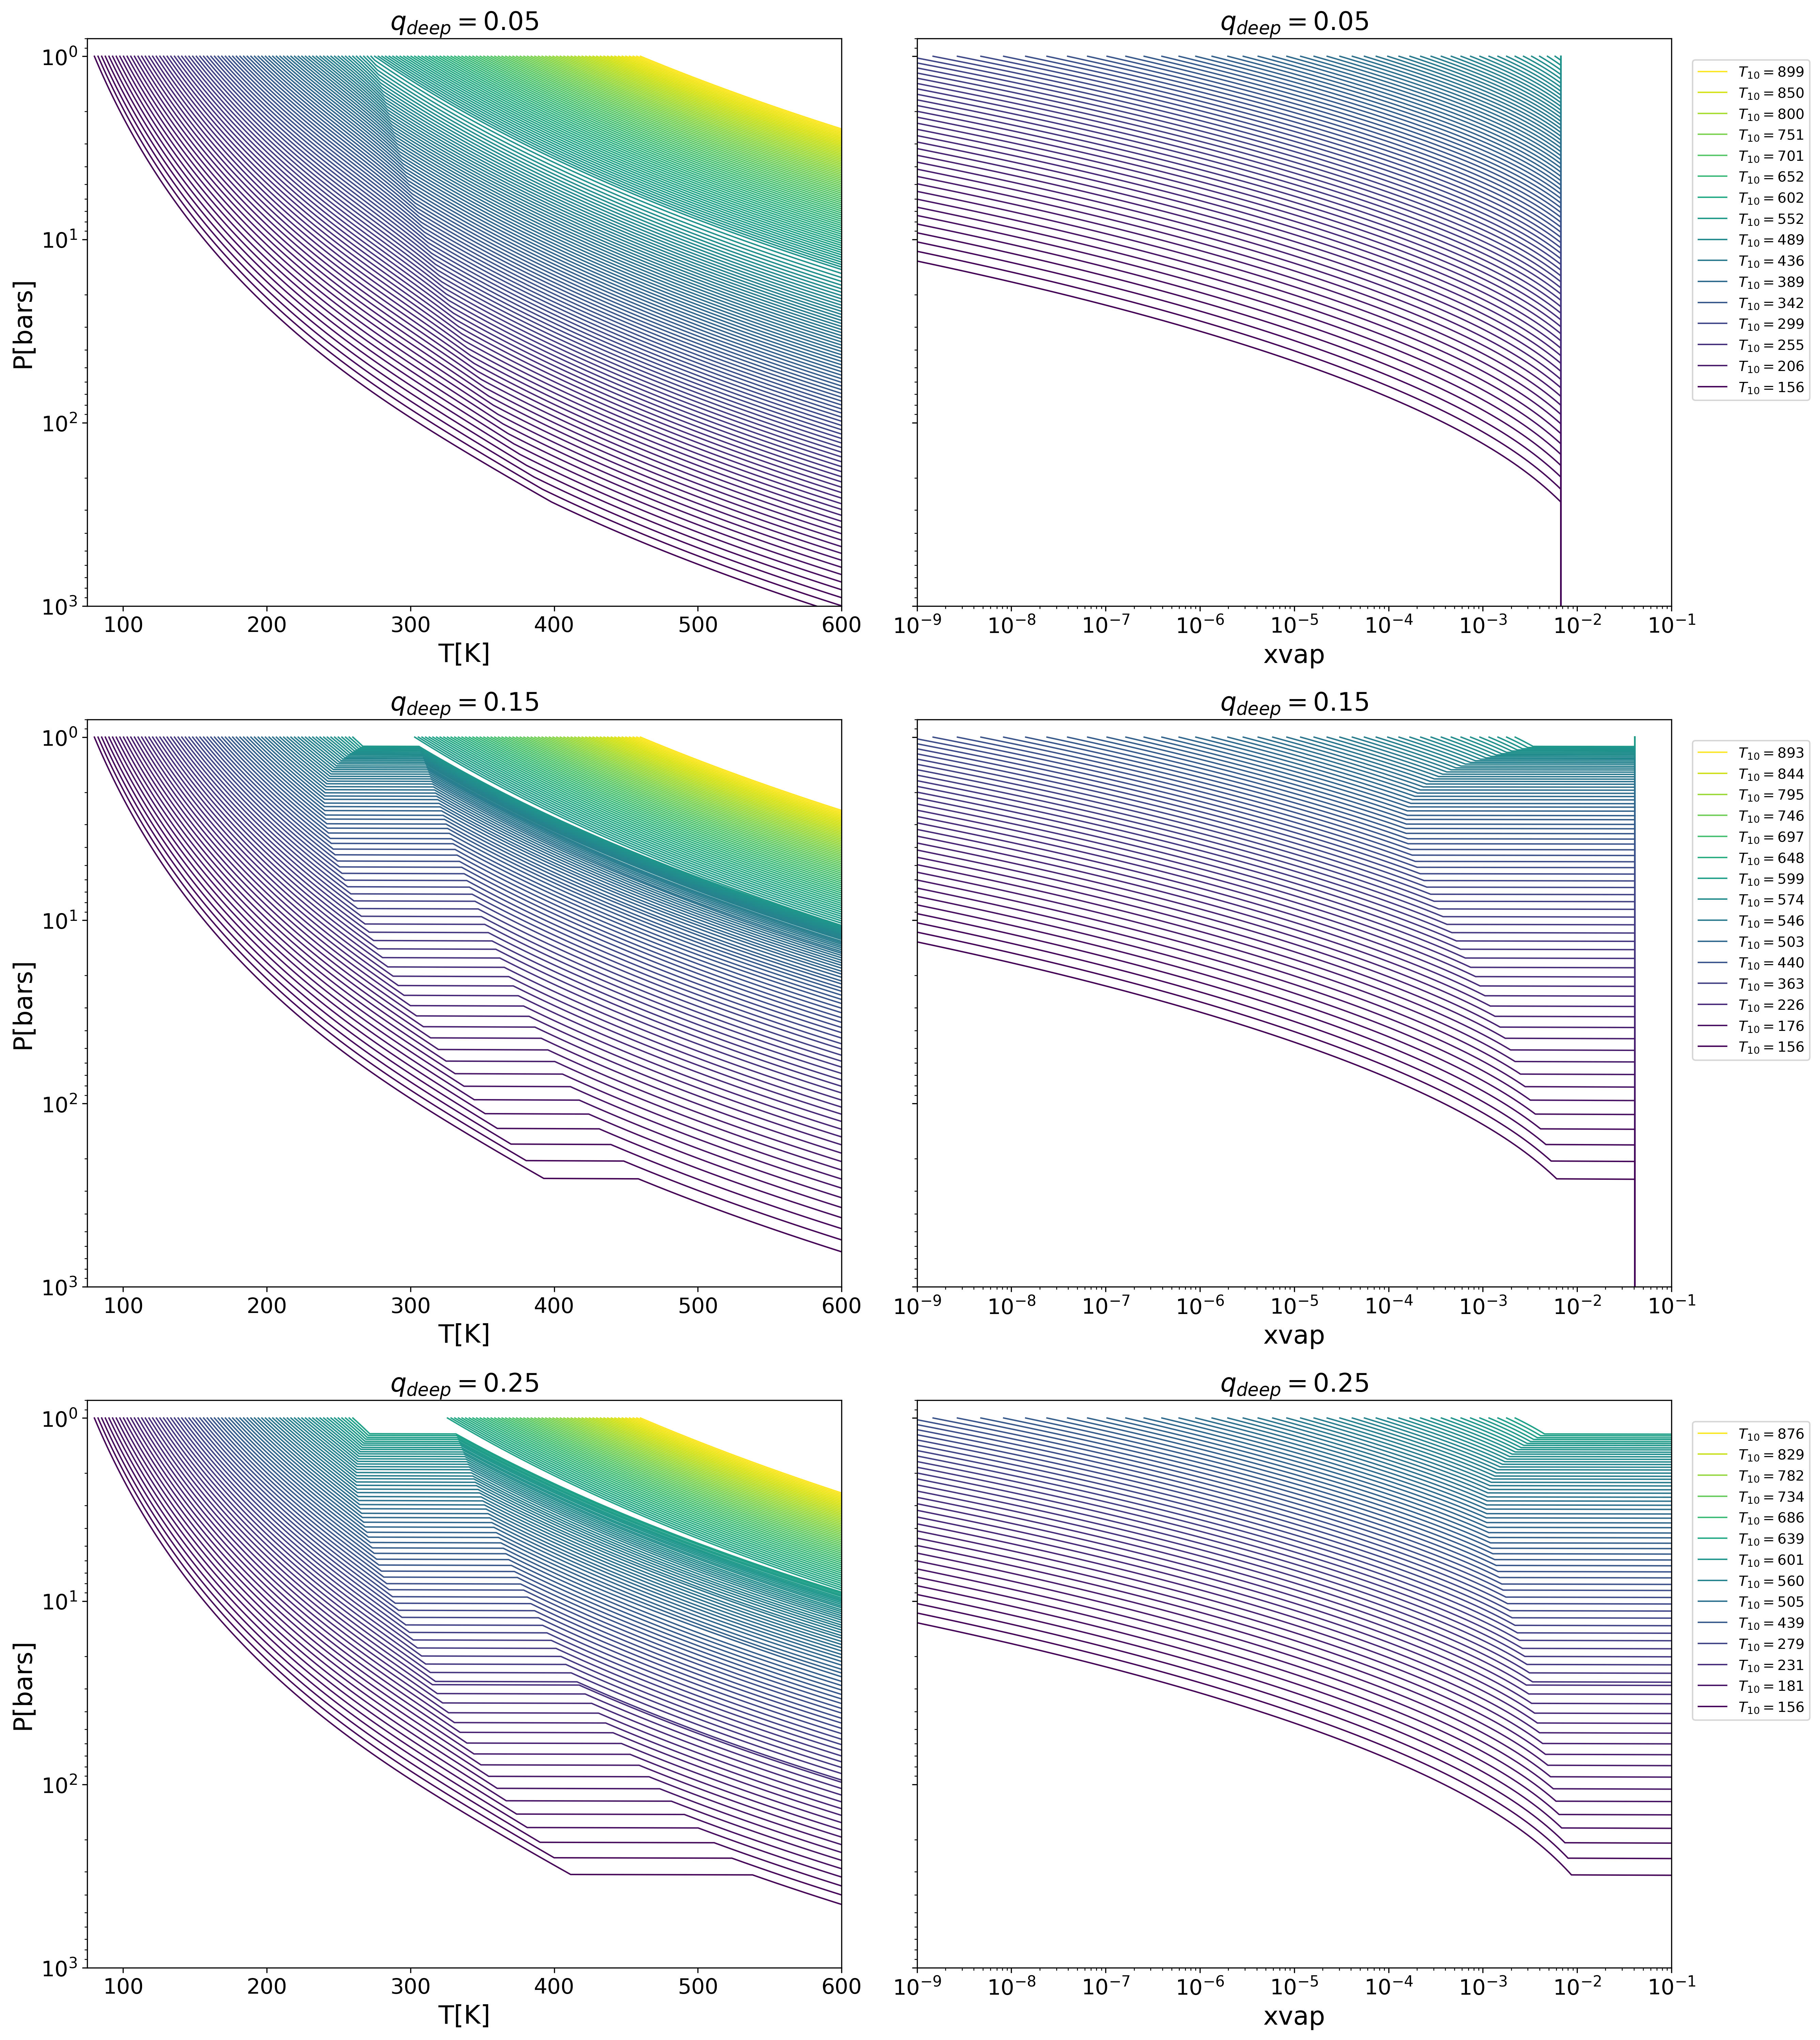
\includegraphics[scale=0.3]{figures/thesis_static_radiative_layer_plots_without_grid_points.png}
 }
\caption[Formation of Radiative Zone]
{These plots were generated using our model Uranus. Again, from top to bottom row, we move from $q_{\rm deep} = 0.05$, $0.15$, and $0.25$, respectively. $T_{10}$'s range from hotter (yellow) to cooler (purple), more recent temperatures. In the top row, no stable radiative zones are formed. The kink visible in the middle of the top left plot represents the transition from a moist to dry adiabat. Condensation occurs, but no stability is achieved. In rows two and three, stable radiative zones are formed, as indicated by the discontinuous temperature jumps moving left to right. The radiative zones form deeper in the interior as the planet cools. The plots in the second column show the vapor mole fraction with respect to pressure. The vapor mole fraction is constant within the radiative zone and reaches its deep water concentration value at the bottom of the radiative zone. }
\label{fig:radiative}
\end{figure}


\section{Thermal Evolution of Uranus and Neptune}

% cooling camparisons of dry adiabat, moist adiabat, and moist adiabat with radiative layer
In Figure~\ref{fig:evolve_adiabats}, we display the results of evolutionary tracks  that considered separately the evolution of a dry adiabat, a moist adiabat with condensation but no stable radiative zone, and a moist adiabat with condensation containing stable radiative zones. For all of these evolutionary tracks, we assumed $q_{\rm deep} = 0.25$. Looking at these evolutionary tracks, the coolest scenario at present time, is a moist adiabat that is never stable against convection. The moist adiabat that is stable against convection has the warmest outcome at present time. In Figure~\ref{fig:evolve_uranus_qdeeps} and Figure ~\ref{fig:evolve_neptune_qdeeps}, we consider the impact of different deep water concentrations on the thermal evolution of Uranus and Neptune, respectively. As the planets cool, their radiative zones descend deeper into the interior, as we saw in Figure~\ref{fig:radiative}. This feature is also noticeable in the thermal evolution plots. Looking at $T_{\rm eff}$ at ~$7 \times 10^7$ Gyr, the onset of condensation-inhibited convection occurs, resulting in a discontinuous temperature drop. The same behavior is seen in the $T_{10}$ plot, however, by this time the radiative zone has descended deeper, later in time at around ~$7 \times 10^8$ Gyr. Larger $q_{\rm deep}$'s result in warmer Uranus and Neptune at present time. We also look at the impact of $q_{\rm deep}$ on the evolution of planetary radius and find that larger values of $q_{\rm deep}$ tend to converge more closely toward the presently observed radius for both Uranus and Neptune in these simulations. [needs more work]

\begin{figure}[ht]
 \centerline{
  \includegraphics[scale=0.5]{figures/dry_moist_radiative_u_cooling_curves_adiabat_comparisons.png}
 }
\caption[Thermal Evolution Curves for Uranus - Adiabat Comparisons]
{The black line represents the thermal evolution for a dry adiabat. The dark red line represents the thermal evolution for a moist adiabat that does not allow for the formation of a stable radiative layer. The light red line represents the thermal evolution of a moist adiabat that does allow for the formation of a stable radiative zone. The fuchsia dot on the lower plot represent the currently observed effective temperature of Uranus with error range. }
\label{fig:evolve_adiabats}
\end{figure}

% cooling uranus
\begin{figure}[ht]
 \centerline{
  \includegraphics[scale=0.45]{figures/u_cooling_curves_nz_4096_more_qdeeps.png}
 }
\caption[Thermal Evolution Curves for Uranus - Water Vapor Concentration Comparisons]
{The curves in these plots represent thermal evolution tracks for different values of $q_{\rm deep}$. Dark blue is the largest concentration of water vapor, at $q_{\rm deep} = 0.55$ and the light blue line is the least concentration of water vapor at $q_{\rm deep} = 0.05$. For $q_{\rm deep} = 0.05$, there is no onset of condensation-inhibited convection and no rapid cooling episode. For larger values of $q_{\rm deep}$ there is a rapid cooling episode for $T_{\rm eff}$ at around $10^8$ Gyr. Similarly, a rapid cooling episode is visible deeper down in the interior as seen in the $T_{10}$ curves at around $10^9$ Gyr. }
\label{fig:evolve_uranus_qdeeps}
\end{figure}

%  cooling neptune
 

\begin{figure}[ht]
 \centerline{
  \includegraphics[scale=0.45]{figures/n_cooling_curves_nz_4096_more_qdeeps.png}
 }
\caption[Thermal Evolution Curves for Neptune - Water Vapor Concentration Comparisons]
{Similar to the Uranus plots, these curves represent cooling tracks for $q_{\rm deep}$'s ranging from $0.05$ to $0.55$. Similar to Uranus, the rapid cooling episodes for $T_{\rm eff}$ and $T_{10}$ occur at $10^8$ Gyr and $10^9$ Gyr, respectively. The vertical fuchsia line in the bottom plot indicates the current observed effective temperature of Neptune [include temp], plus or minus [include temp error] }
\label{fig:evolve_neptune_qdeeps}
\end{figure}



%  cooling radius curves
\begin{figure}[ht]
 \centerline{
  \includegraphics[scale=0.45]{figures/u_cooling_radius_nz_4096_logx_more_qdeeps.png}
 }
\caption[Thermal Evolution Curves for Uranus - Radius]
{This thermal evolution plot shows the impact of different deep water concentration on the radius as the planet cools. The gray square represents the current observed radius.}
\label{fig:evolve_uranus_radius}
\end{figure}


\begin{figure}[ht]
 \centerline{
  \includegraphics[scale=0.45]{figures/n_cooling_radius_nz_4096_logx.png}
 }
\caption[Thermal Evolution Curves for Neptune - Radius]
{[Combine this plot with the above and have one caption.] }
\label{fig:evolve_neptune_radius}
\end{figure}



\chapter{Discussion and Conclusions}
We set out to investigate the impact of water condensation zones on the thermal evolution of our solar system ice giants. It has been speculated that such thermal boundary layers could act as an imperfect insulator, trapping heat below and allowing the envelope above the boundary layer to cool more rapidly \citep{nettelmann_2016}\citep{friedson_2017}\citep{leconte_2017}\citep{podolak_1991}\citep{scheibe_2019}. It seems plausible that interiors containing these thermal boundary layers could explain the problem with Uranus appearing to have no intrinsic temperature. Our findings are inconclusive. We do find that incorporating a moist adiabat into our interior structure model does result in a cooler planet than would otherwise be seen with a purely dry model. However, when we add stable radiative zones to the interior, we do find in the planet's past a period of rapid cooling that results in a cooler effective temperature at around $10^8$ Gyr, the planet eventually becomes warmer at present time than predicted by dry or simple moist adiabatic models. Reality is certainly more complex than the assumptions upon which our model is based. It is quite possible that reality resembles something in between the binary choice of a moist adiabat with or without thermal boundary layers\citep{guillot_2019}. Our assumption of a stable shell of water condensation assumes that there are no other dynamics at play, such as upwelling or entrainment pressure \citep{friedson_2017} eroding and punching holes in the stable radiative zone. Such scenarios could allow for more mixing of the warm gases below and above the condensation zone. We also considered only one condensate, H$_{2}$O. It would be worth considering $NH_{3}$ and $CH_{4}$, and analyzing the impact of multiple stratified layers on the cooling of the planet over time.





\newcommand{\newblock}{}
\bibliography{wcz_bib}


\end{document}
